\begin{artengenv2auth}{Roman Krzanowski, Pawel Polak}
	{The meta-ontology of AI systems with human-level intelligence}
	{The meta-ontology of AI systems with human-level intelligence}
	{The meta-ontology of AI systems with human-level intelligence}
	{\textsuperscript{1}Departments of Philosophy and Mathematics, Carnegie Mellon University\\
		\textsuperscript{2}Copernicus Center for Interdisciplinary Studies, Jagiellonian University}
	{\label{krzanowpolak_start}In this paper, we examine the meta-ontology of AI systems with human-level intelligence, with us denoting such AI systems as AI\textsubscript{E}. Meta-ontology in philosophy is a~discourse centered on ontology, ontological commitment, and the truth condition of ontological theories. We therefore discuss how meta-ontology is conceptualized for AI\textsubscript{E} systems. We posit that the meta-ontology of AI\textsubscript{E~}systems is not concerned with computational representations of reality in the form of structures, data constructs, or computational concepts, while the ontological commitment of AI\textsubscript{E} systems is directed toward what exists in the outside world. Furthermore, the truth condition of the ontology (which is meta-ontological assumption) of AI\textsubscript{E} systems does not require consistency with closed conceptual schema or ontological theories but rather with reality, or in other words, ``what is the world''
	%\label{ref:RNDuTcZpb4G1k}(Smith, 2019, p.57).
	\parencite[][p.57]{smith_promise_2019}. %
	 In addition, the truth condition of AI\textsubscript{E} systems is verified through operational success rather than by coherence with theories. This work builds on ontological postulates about AI systems that were formulated by Brian Cantwell Smith 
	%\label{ref:RND1W3b57kSJx}(2019).
	\parencite*[][]{smith_promise_2019}.%
	}
	{human-level intelligence AI, meta-ontology of AI Paradigm, AI Paradigm, ontology of AI Paradigm, ontological commitment of AI Paradigm, John Haugeland, Brian Cantwell Smith, Marvin Minsky, Hubert Dreyfus.}
	{%
%		{\flushright\subbold{Roman Krzanowski}\\\subsubsectit\small{Pontifical University of John Paul II in Krakow}\par}%
%		{\flushright\subbold{Pawel Polak}\\\subsubsectit\small{Pontifical University of John Paul II in Krakow}\par}%
		{\flushright\subbold{Roman Krzanowski}\\\subbold{Pawel Polak}\\\subsubsectit\small{Pontifical University of John Paul II in Kraków, Poland}\par}%
	}



%\begin{document}
%\title{The meta-ontology of AI systems with human-level intelligence}
%\maketitle
%
%\section*{Abstract}
%In this paper, we examine the meta-ontology of AI systems with human-level intelligence, with us denoting such AI systems as AI\textsubscript{E}. Meta-ontology in philosophy is a~discourse centered on ontology, ontological commitment, and the truth condition of ontological theories. We therefore discuss how meta-ontology is conceptualized for AI\textsubscript{E} systems. We posit that the meta-ontology of AI\textsubscript{E~}systems is not concerned with computational representations of reality in the form of structures, data constructs, or computational concepts, while the ontological commitment of AI\textsubscript{E} systems is directed toward what exists in the outside world. Furthermore, the truth condition of the ontology (which is meta-ontological assumption) of AI\textsubscript{E} systems does not require consistency with closed conceptual schema or ontological theories but rather with reality, or in other words, ``what is the world''
%%\label{ref:RNDuTcZpb4G1k}(Smith, 2019, p.57).
%\parencite[][p.57]{smith_promise_2019}. %
% In addition, the truth condition of AI\textsubscript{E} systems is verified through operational success rather than by coherence with theories. This work builds on ontological postulates about AI systems that were formulated by Brian Caldwell Smith 
%%\label{ref:RND1W3b57kSJx}(2019).
%\parencite*[][]{smith_promise_2019}.%
%
%
%Keywords: \textit{human-level intelligence AI, meta-ontology of AI Paradigm, AI Paradigm, ontology of AI Paradigm, ontological commitment of AI Paradigm, J. Haugeland, B. C. Smith, M. Minsky, H. Dreyfus.}

\section*{Introduction}
\lettrine[loversize=0.13,lines=2,lraise=-0.07,nindent=5pt,findent=-5pt]%
{A}{}rtificial intelligence systems have developed over the past 60 years, bringing new solutions to a~huge number of practical problems, and they continue to find many surprising and fascinating applications. However, the main goal of AI, namely the creation of a~human-like intelligence,\footnote{See ft. 3 on AGI for an explanation of human-like intelligence.} is still proving unattainable. Indeed, the
AI systems we currently design and implement cannot replicate human intelligence and a~human agent's ability to cope with reality
%\label{ref:RNDzbUfjwINVD}(see e.g. Brooks, 1991; Minsky, 1991; Dreyfus, 2016; Mitchell, 2019; Bołtuć, 2020; Roitblat, 2020; Wooldridge, 2021).
\parencites[see, e.g.,][]{brooks_intelligence_1991}[][]{minsky_logical_1991}[][]{dreyfus_skillful_2016}[][]{mitchell_artificial_2019}[][]{boltuc_conscious_2020}[][]{roitblat_algorithms_2020}[][]{wooldridge_road_2021}.%


One of the reasons for this failing (in their ability to cope with reality) is, it seems, related to how these AI systems lack a~proper ontology or representation of the real world. (For more about the failings of current AI conceptualizations, see, for example, the works of Brooks
%\label{ref:RNDRn6fjQo5fK}(1991),
\parencite*[][]{brooks_intelligence_1991}, %
 Dreyfus 
%\label{ref:RNDQXX8Yv0mJq}(2016),
\parencite*[][]{dreyfus_skillful_2016}, %
 and Smith 
%\label{ref:RNDVD6ttaHRwZ}(2019)
\parencite*[][]{smith_promise_2019}%
).\footnote{To get a~sense of the ontologies (and meta-ontologies) of the real world in biological agents, consult Ed Yong's book \textit{An Immense World} 
%\label{ref:RNDQEaQIHeWBf}(Yong, 2022).
\parencite[][]{yong_immense_2022}. %
Interesting analysis of deep learning systems ontological commitments see
%(Šekrst and Skansi, 2022).
\parencite[][]{sekrst_machine_2022}.} %
Smith 
%\label{ref:RNDAN4wrT01Ck}(2019, p.44)
\parencite*[][p.44]{smith_promise_2019} %
 proposed four features that AI systems should possess if they are to mimic humans' ability to cope with the real world (i.e., have human-level intelligence). These systems, which we here refer to as AI\textsubscript{E} systems, should be embodied, embedded, extended, and enactive 
%\label{ref:RND7XiVNpc9Oj}(see also Käufer and Chemero, 2021).
\parencite[see also][]{kaufer_phenomenology_2021}. %
 While these features are not ontological per se, but they do imply a~commitment to some ontology. What the kind of ontology these four features would entail is a~meta-ontological question that we explore in this paper, thus furthering the ideas studied by Krzanowski and Polak 
%\label{ref:RNDbpbe9vUMPT}(2022).
\parencite*[][]{krzanowski_ontology_2022}.%


This paper is organized as follows: First, we define some basic concepts related to the meta-ontological discourse, namely ontology, specifically ontology of computing and AI systems, meta-ontology, ontological commitment, and truth conditions. As these concepts have many interpretations, we need precise definitions to ensure that the subsequent discussion will be understood as intended. Next, we explain the main postulates of meta-ontology for AI\textsubscript{E} systems, the topic of this work. In the conclusion, we discuss the inherent limitations of ontologies (which is a~meta-ontological problem) for artificial systems such as AI\textsubscript{E}, their inability to match human intelligence, and the potential prospects for AI\textsubscript{E}. (For more on the problems of ontology in AI systems see, for example, Haugeland
%\label{ref:RNDYBbHi2hgVs}(1985)
\parencite*[][]{haugeland_artificial_1985} %
 and Fjelland 
%\label{ref:RNDnEqrE2ShbQ}(2020)
\parencite*[][]{fjelland_why_2020}%
).

Three things should be borne in mind while reading this paper. First, AI systems with human-level intelligence are often referred to as AGI systems, but with many interpretations for this concept, we avoid using this term to prevent us from drifting into the debate about AGI.\footnote{See various references for different conceptualizations of AGI
%\label{ref:RNDlE6bxZSweV}(e.g. Mitchell, 2019, p.40; Fjelland, 2020);
\parencites[e.g.,][p.40]{mitchell_artificial_2019}[][]{fjelland_why_2020}; %
 general purpose, human-level intelligence 
%\label{ref:RNDTtFTF8X0Xa}(Marcus, 2022);
\parencite[][]{marcus_artificial_2022}; %
 the generic ability of a~machine to consciously perform any task that a~human can 
%\label{ref:RND1RaLeokAOz}(Kumpulainen and Terziyan, 2022);
\parencite[][]{swar_unified_2022}; %
 the intelligence of a~machine that is capable of understanding the world 
%\label{ref:RND3vayfssWih}(Skuza, 2020);
\parencite[][]{skuza_what_2020}; %
 the representation of generalized human cognitive abilities 
%\label{ref:RNDtYCoFCClKk}(Lutkevich, 2022);
\parencite[][]{lutkevich_what_2022}; %
 a~general-purpose capability, including the ability to broadly generalize to fundamentally new areas 
%\label{ref:RNDQOScPjMeEk}(Cassimatis, Bello and Langley, 2008);
\parencite[][]{cassimatis_ability_2008}; %
 and the capacity of an engineered system to display the same rough sort of general intelligence as humans 
%\label{ref:RNDbpu6DOErGB}(Goertzel, 2015).
\parencite[][]{goertzel_artificial_2015}. %
 Creating human-level intelligence was always the aim of AI research, as attested to by Yann LeCun's recent claim ``Getting machines to behave like humans and animals has been the quest of my life'' (reported in \emph{\textup{2022 MIT Technology Review }}\label{ref:RNDzntlMH5EtX}\emph{\textup{(Heikkil}}ä and Heaven, 2022)\emph{\textup{)}.}} Second, this is a~study of the meta-ontology of specific AI systems, i.e., AI\textsubscript{E}, meaning that the focus of the study is ontology of these AI systems rather than philosophical ontology. Philosophy forms the background of this discussion, but it is not its main objective. Third, we are not concerned with particular implementations of AI\textsubscript{E} systems, which is why we instead study the AI\textsubscript{E} system paradigm, which is the all-encompassing conceptual framework of AI\textsubscript{E} systems that supports multiple implementations. Thus, when we talk about an AI\textsubscript{E} system, we are referring to an AI\textsubscript{E} system paradigm rather than a~specific implementation. The concept of AI paradigm and its role in this study are explained later in the paper.

\section*{Key grounding ideas}
\subsection*{The ontology of AI}

Ontology can be thought as an empty buzzword or a~specific conceptual construct,\footnote{``We must be careful in reading [auth. any] philosophical works on ontology, when the author speaks of ‘ontology' without qualifications, not to confuse the intended sense of the world with any of the alternatives''
%\label{ref:RNDfLy5S3W893}(Jacquette, 2002, p.3).
\parencite[][p.3]{jacquette_ontology_2002}. %
 There is also a~confusion between ontology and metaphysics. Some authors see ontology as the ultimate study of reality 
%\label{ref:RNDvlH3CHHmmY}(e.g. Jacquette, 2002; Stróżewski, 2004, p.32, or Perzanowski, 2015),
\parencites[e.g.,][]{jacquette_ontology_2002}[][]{strozewski_ontologia_2004}[or][]{perzanowski_rozprawa_2015}, %
 and metaphysics as being ``after physics'', some others see ontology as a~part of metaphysics 
%\label{ref:RNDeDepxi7xRN}(see e.g. Van Inwagen, 2009).
\parencite[see e.g.,][]{van_inwagen_metaphysics_2009}. %
 In AI literature because ontology takes on a~very concrete garb (of an engineering domain) metaphysics is a~rare term so the confusion is not so visible.} so we need to position the ontology of AI\textsubscript{E~}within the world of ontological theories and demonstrate, what it means in this discussion, how it relates to ``other'' ontologies in philosophy, computer science, and AI. Ontology in computer science and AI systems 
%\label{ref:RNDxG2UeatxFk}(e.g. Sánchez, Cavero and Martínez, 2007; as well Guarino and Giaretta, 1995; Guarino, Oberle and Staab, 2009; Swar, Khoriba and Belal, 2022)
\parencites[e.g.,][]{sharman_road_2007}[as well][]{guarino_ontologies_1995}[][]{guarino_what_2009}[][]{swar_unified_2022} %
 takes on different meanings to that of philosophy 
%\label{ref:RNDWOSOcJkOvq}(e.g. Jacquette, 2002; Stróżewski, 2004; Baker, 2007; Chalmers, Wasserman and Manley, 2009; Effingham, 2013; Berto and Plebani, 2015; Perzanowski, 2015; Thomasson, 2015; Hofweber, 2021).
\parencites[e.g.,][]{jacquette_ontology_2002}[][]{strozewski_ontologia_2004}[][]{baker_metaphysics_2007}[][]{chalmers_metametaphysics_2009}[][]{effingham_introduction_2013}[][]{berto_ontology_2015}[][]{perzanowski_rozprawa_2015}[][]{thomasson_ontology_2015}[][]{hofweber_logic_2021}.%
\footnote{Importing AI (or technical) aspects into philosophy brings with it a~touch of reality that philosophical considerations often lack. See also the comment by Jacquette on the relation between a~domain ontology and the domain itself 
%\label{ref:RNDY4CVeRGcfL}(Jacquette, 2002, p.5).
\parencite[][p.5]{jacquette_ontology_2002}.%
} The philosophical concepts of ontology, however, are fundamental to those used in specific applications 
%\label{ref:RNDFJ4JNj0TbG}(see the comments of Jacquette, 2002, p.XII).
\parencite[see the comments of][p.XII]{jacquette_ontology_2002}. %
 This is therefore where we begin.

In philosophy, ontology is the study of being as it is (i.e., ``what is''), so it is about ``being'' in the most general sense.\footnote{The term ``being'' is used in the sense employed by the Ancient Greeks, Parmenides (opposite to The Unbeing), Aristotle (Being qua being), medieval scholars like Aquinas (the study of being qua being)
%\label{ref:RNDFR1vKzYSIx}(Kerr, 2022),
\parencite[][]{kerr_aquinas_2022}, %
 and some modern philosophers such as 
%\label{ref:RNDYFnNv0y86Z}(Jacquette, 2002; Stróżewski, 2004, p.32, or Perzanowski, 2015).
\parencites[][]{jacquette_ontology_2002}[][]{strozewski_ontologia_2004}[or][]{perzanowski_rozprawa_2015}. %
 This term is also sometimes written as Being meaning totality of what exist 
%\label{ref:RNDjNhA4sxPMl}(Kenny, 2012, p.160).
\parencite[][p.160]{kenny_new_2012}. %
 Many modern philosophies, scientists computer engineers infuse this term with many different meanings (see this paper for the examples) obfuscating the original Greek sense of \textit{onto-logia} -- the fundamental study of being, probably as too esoteric (i.e., metaphysical) for their tastes 
%\label{ref:RNDjJRKpH1qcI}(see also Kenny, 2012; Hofweber, 2021).
\parencites[see also][]{kenny_new_2012}[][]{hofweber_logic_2021}.%
} More specifically, in its purely philosophical meaning, ontology is the study of the foundations of what exists, what is common and most general among it, and what its origins are 
%\label{ref:RNDfYYNHUcznT}(see e.g. Jacquette, 2002; Stróżewski, 2004, p.32)
\parencites[see, e.g.,][]{jacquette_ontology_2002}[][p.32]{strozewski_ontologia_2004}. %
 Hereafter, we refer to this concept by a~boldface, capital ``O'' without a~subscript (i.e., \textbf{O}).

Ontology in philosophy may also refer to ``what exists'' in a~much more constrained, narrower, sense. This kind of ontology investigates existing, subject to a~definition for existence, objects and relations in the world, and we will refer to this ontology as O. Depending on the assumptions made, different types of objects and relations may be recognized by O~ontologies, because O~branches into many subdomains. Thus, many different perspectives have been developed for ontology
%\label{ref:RNDJ0HiQvGuma}(e.g. Quine, 1960; Jacquette, 2002; Stróżewski, 2004; Baker, 2007; Chalmers, Wasserman and Manley, 2009; Effingham, 2013; Ingarden, 2013; 2016; Berto and Plebani, 2015; Perzanowski, 2015; Thomasson, 2015; Hofweber, 2021);
\parencites[e.g.,][]{quine_word_1960}[][]{jacquette_ontology_2002}[][]{strozewski_ontologia_2004}[][]{baker_metaphysics_2007}[][]{chalmers_metametaphysics_2009}[][]{effingham_introduction_2013}[][]{ingarden_controversy_2013}[][]{ingarden_controversy_2016}[][]{berto_ontology_2015}[][]{perzanowski_rozprawa_2015}[][]{thomasson_ontology_2015}[][]{hofweber_logic_2021}; %
 these differ in terms of extent, content, consistency, and accuracy, often responding to the specific needs of a~domain.

In computational systems, ontology can be defined as ``a specific vocabulary (dictionary) used to describe a~certain reality, plus a~set of explicit assumptions regarding the intended meaning of the vocabulary words''
%\label{ref:RNDAcXPc7BmPe}(see Guarino and Giaretta, 1995; Guarino, Oberle and Staab, 2009).
\parencites[see][]{guarino_ontologies_1995}[][]{guarino_what_2009}. %
 In this context, ontologymay also refer to ``a model of the structure of a~system'' 
%\label{ref:RNDi9mTVDxk3A}(Guarino, Oberle and Staab, 2009)
\parencite[][]{guarino_what_2009} %
 or ``a formal, explicit specification of a~shared conceptualization'' 
%\label{ref:RNDAqesK2fTKs}(Studer, Benjamins and Fensel, 1998).
\parencite[][]{studer_knowledge_1998}. %
 We also have computational ontologies, which often called engineering ontologies, that ``are machine-processable structures which represent particular domains of interest'' 
%\label{ref:RNDiOONhTuWRW}(Husáková and Bureš, 2020).
\parencite[][]{husakova_formal_2020}. %
 Ontology may also be used to refer to knowledge-based systems, databases, or AI systems that manage knowledge bases 
%\label{ref:RND7tN9yeZ52M}(see the discussions of Sharman, Kishore and Ramesh, 2007; Staab and Studer, 2009; Garbacz and Oliver Kutz, 2014; Husáková and Bureš, 2020).
\parencites[see the discussions of][]{sharman_ontologies_2007}[][]{staab_handbook_2009}[][]{garbacz_formal_2014}[][]{husakova_formal_2020}.%


The ontology of AI\textsubscript{E} systems, meanwhile, denotes and determines how an AI\textsubscript{E} system represents and reasons about the real world. Itis not concerned with computational representations of reality through structures, theories, data constructs, or computational concepts but rather with how real world objects, properties, and relations are registered by an AI system, as well as how they are recognized and interpreted. In brief, this ontology is solely committed to the real world
%\label{ref:RNDHoOzRM31HN}(in the sense explained by Smith, 2019, p.145),
\parencite[in the sense explained by][p.145]{smith_promise_2019}, %
 with it reflecting the real world\footnote{The term ``real world'', or reality, is understood here as it is understood in Smith 
%\label{ref:RNDdF84GECegW}(2019, pp.xiii, xiv),
\parencite*[][xiv]{smith_promise_2019}, %
 denoting the physical world we live in. Minsky 
%\label{ref:RND166uXGx81U}(1991, p.6)
\parencite*[][p.6]{minsky_logical_1991} %
 refers to this reality as common sense reality. The term may be opposed to ``virtual worlds'', ``imaginary worlds'', ``fantastic worlds'', or other qualified uses of ``words'' denoting worlds as creations of computer systems, artistic expressions, or imaginations. The term ``world'' or ``real world'' may have multiple interpretations that we have no intention to discuss as such a~discussion would be pointless and would not further the main point of the paper. Thus, the reader seeking more detailed explanation of this term should follow the cited references.}, or physical reality, and the AI system's place in this world. More specifically, it is embodied, embedded, extended, and enactive 
%\label{ref:RNDcx3KAaKj2v}(Smith, 2019, p.43),
\parencite[][p.43]{smith_promise_2019}, %
 which are terms that will be explained later in this paper. There is no formal theory to accompany 4E ontology (ontology of AI system that is embodied, embedded, extended, and enactive), so there are no criteria for theoretical truth verification, but verification comes instead from a~confrontation with the real world, which we will discuss later. A~4E ontology is not given in the form of a~set of a~priori relations and objects but rather acquired 
%\label{ref:RNDIdA3C5UrQl}(Smith, 2019)
\parencite[][]{smith_promise_2019} %
 in response to a~dynamically changing reality 
%\label{ref:RNDjzZunSO8Xh}(see Minsky, 1991, as well as; Bołtuć, 2020).
\parencites[see][as well as]{minsky_logical_1991}[][]{boltuc_conscious_2020}. %
 We will refer to this ontology as O\textsubscript{E}.

Let us now put these things together. Ontology (\textbf{O}), as a~philosophical discipline, asks what is, in a~most general sense, and what exists Ontology (O) is more restricted with the scope of this ontology being defined by the horizon of interest: For example, it may be the universe, some aspect of it, or a~domain of reality (i.e., domain ontology), like ontology of biology, or ontology of physics. Ontology in computational systems, meanwhile, can be defined as ``a specific vocabulary used to describe a~certain reality, plus a~set of explicit assumptions regarding the intended meaning of the vocabulary entries,'' while the ontology of AI systems relates specifically to a~representation of the world or some knowledge domain in AI systems. Finally, the ontology of an AI\textsubscript{E} system (O\textsubscript{E}) refers to how AI\textsubscript{E} system represents about the real world and how it is situated within reality.

Figure \ref{krz-ill1} illustrates these ontological dependencies by showing them in terms of their increased specificity both in scope as well as in application domain, from the most general (\textbf{O}), which is the ontology of what exists (O), to the most specific one, which in this case is O\textsubscript{E}, the ontology of an AI\textsubscript{E} system.



%\begin{figure}[htp]
%\centering
%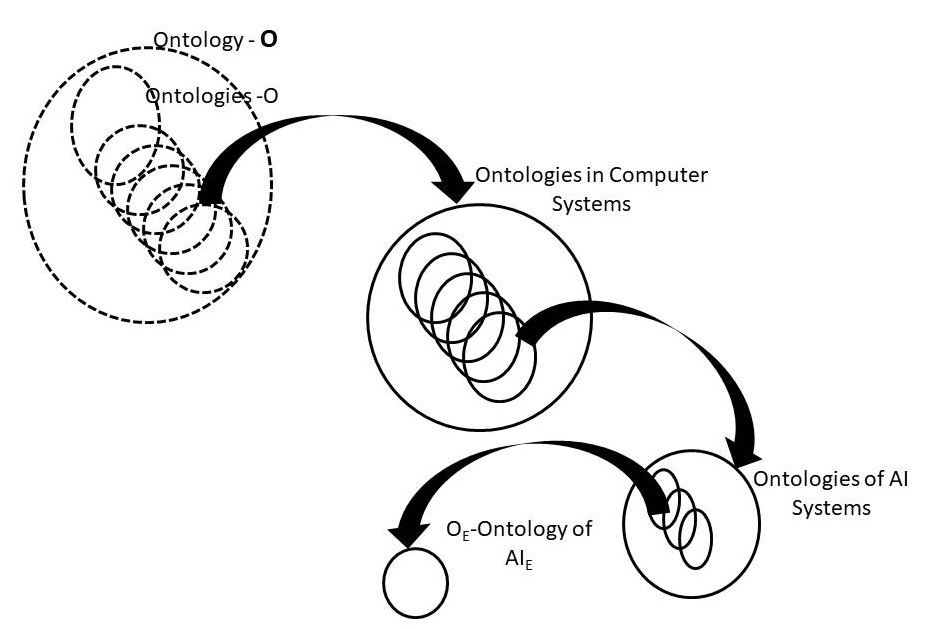
\includegraphics{ART_Krzanowski_Polak/Ontology2200B_pu.jpg}
%\end{figure}
%Figure 1. AI\textsubscript{E} ontology and hierarchy of ontologies.

\begin{figure}[htp]
 \begin{center}
 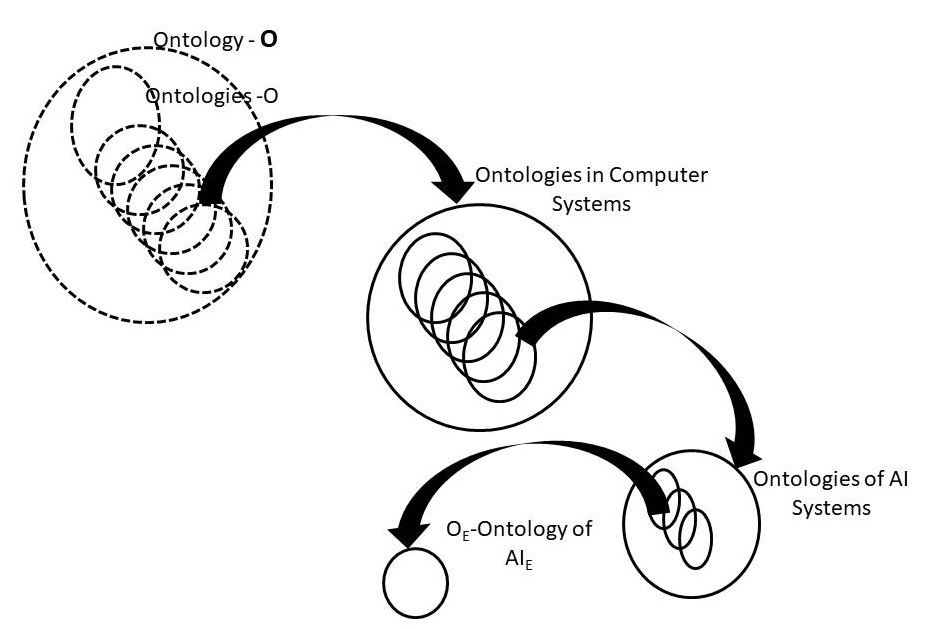
\includegraphics[width=.9\textwidth]{ART_Krzanowski_Polak/Ontology2200B_pu.jpg}%
 \end{center}%
 \caption{AI\textsubscript{E} ontology and hierarchy of ontologies.}\label{krz-ill1}
\end{figure}


Thus, with respect to specificity and scope, O\textsubscript{E} falls under the AI ontologies, which in turn are subspecies of the ontologies of computer systems, and these in turn are forms of specific ontologies (O) concerned with a~specific segment of reality, which then falls under fundamental ontology (\textbf{O}) for existence. All these ontologies ask the same question but within different contexts, scopes, and perspectives. Furthermore, Figure \ref{krz-ill1} shows how only ontology \textbf{O} attempts to comprehend all that exists, with other ontologies being mere fragments. The further away we move from the fundamental ontology \textbf{O}, the narrower and more specific the scope of the ontology becomes.

%Thus, ontology that represents the real world being always expressed in some form of language (which always is) is always incomplete with respect to the world, i.e., the world ``as is'' cannot be represented by something else, despite the close isomorphism between the reality and some logical aka ontological systems \footnote{All pure ontological systems are logical systems
%%\label{ref:RNDQXsIfZlLYA}(Jacquette, 2002, p.xiii; see e.g. Foschini, 2013).
%\parencites[][p.xiii]{jacquette_ontology_2002}[see, e.g.,][]{foschini_where_2013}.%
%}

%%%%%%%%%%%%%%%%%%%%%%%%%%%%%%%%%%%%



Thus, ontology that represents the real world being always expressed in some form of language (which always is) is always incomplete with respect to the world, i.e., the world ``as is'' cannot be represented by something else, despite the close isomorphism between the reality and some logical aka ontological systems.\footnote{All pure ontological systems are logical systems
%\label{ref:RNDQXsIfZlLYA}(Jacquette, 2002, p.xiii; see e.g. Foschini, 2013).
\parencites[][p.xiii]{jacquette_ontology_2002}[see e.g.,][]{foschini_where_2013}.%
} As a~result, there will always be some inconsistency between what exists and what a~given ontology represents, because ontology (even ontology \textbf{O}) will always be a~theory (of sorts), expressed in some specialized language (see ft. 8) about the world rather than the world itself. Thus, there will always be a~degree of incommensurability,\footnote{Incommensurability is not understood here in the same way as the incommensurability of paradigms or scientific theory in the works of Khun 
%\label{ref:RNDg7lp3HNe18}(1962)
\parencite*[][]{kuhn_structure_1962} %
 or Feyerabend 
%\label{ref:RNDdDGQ3TRwiM}(e.g. Ryan, 2002; Sankey, 1993; Oberheim and Hoyningen-Huene, 2018; Bird, 2000).
\parencites[e.g.,][]{ryan_feyerabend_2002}[for the incommensurability of paradigms, see also][]{sankey_kuhns_1993}[][]{oberheim_incommensurability_2018}[][]{bird_thomas_2000}. %
 Instead, incommensurability is understood here as a~general sense of not being entirely comparable according to some criteria.} or a~gap, between the ontology of synthetic systems and the reality of what exists. This gap may be narrowed but never entirely closed. Indeed, a~representation can never contain itself as a~part of what exists. We should keep this incommensurability in mind when building synthetic systems like~AI\textsubscript{E}.

\subsection*{The meta-ontology of AI}

Meta-ontology is a~relatively recently coined term with many interpretations. In philosophy meta-ontology denotes a~study of ontology, what it investigates, and what it is concerned with
%\label{ref:RNDOe0O2QLaGe}(e.g. Quine, 1960; Eklund, 2008; Berto and Plebani, 2015).
\parencites[e.g.,][]{quine_word_1960}[][]{eklund_picture_2008}[][]{berto_ontology_2015}. %
 Peter Van Inwagen 
%\label{ref:RNDlQ2vAbyD19}(1998),
\parencite*[][]{van_inwagen_meta-ontology_1998}, %
 the originator of the term, posited that the role of meta-ontology is to clarify the subject of ontology and explain how ontological claims can be interpreted. Francesco Berto and Matteo Plebani describe meta-ontology in terms of ``‘meta-X' as the inquiry on the central concepts and procedures of discipline X'' 
%\label{ref:RNDRhsH36U3p0}(Berto and Plebani, 2015, p.13),
\parencite[][p.13]{berto_ontology_2015}, %
 where ``X'' refers to ontology in this case. Meta-ontology asks what a~philosopher means when he asks ontological questions or questions about ontology 
%\label{ref:RND0XCU1LJYrl}(Eklund, 2008; Turner, 2014).
\parencites[][]{eklund_picture_2008}[][]{turner_metaontology_2014}. %
 Furthermore, meta-ontology is also concerned with ontological commitments and the truth conditions for a~given ontological theory 
%\label{ref:RNDPFqAz4nWnW}(Van Inwagen, 1998).
\parencite[][]{van_inwagen_meta-ontology_1998}. %
 From this perspective, meta-ontology would inquire as to what kind of ``things'' an ontological theory (i.e., ontology) is committed to.\footnote{We do not discuss Quine's meta-ontology as being specific to Quine's concept of ontology that is not considered here.}

Ontological commitment and truth condition are key terms for defining meta-ontology, and they are critical for differentiating between ontology and meta-ontology
%\label{ref:RNDIMrAPRSpV1}(Turner, 2014).
\parencite[][]{turner_metaontology_2014}. %
 On the conceptual level, the ontological commitment denotes what kind of ontology (i.e., what exists, what is) a~system or a~theory is supposed to represent. Gibson 
%\label{ref:RNDSpom5lKiCH}(2009, p.631)
\parencite*[][p.631]{gibson_ontological_2009} %
 states that ``theory is ontologically committed to an object only if that object occurs in all the ontologies of that theory.'' Thus, ontology may be committed to the existence of numbers, planets, subatomic particles, ghosts, values, ethics, and so on, anything as long as these ``things'' are recognized in ``all the ontologies of that theory'' 
%\label{ref:RND0EJlQmQ9Dk}(e.g. Eklund, 2008).
\parencite[e.g.,][]{eklund_picture_2008}. %
 While ontology is about existence, ``what is'', the ontological commitment is about representation of ``what is'' 
%\label{ref:RNDvi3QcENC1N}(Smith, 1998)
\parencite[][]{smith_origin_1998} %
 and the capacity to represent it.

Moreover, ontological commitment also includes verifying the criteria for this ontological commitment (i.e., verifying the truth of its existential claims). Ontological commitment can be reduced to the simple claim that ``A man is committed to the truth of whatever he asserts''
%\label{ref:RNDA5OgzdmbIa}(Searle, 1969, p.112).
\parencite[][p.112]{searle_speech_1969}.%
\footnote{See the critique of Searle by Inwagen
%\label{ref:RNDdyJS6eDQgJ}(Inwagen, 1991).
\parencite*[][]{lepore_searle_1991}.%
} For some, however, particularly professional ontologists, Searle's take on ontological commitment seems perfunctory, but in the AI context, it provides a~simple (i.e., operational) means for judging the scope of an AI ontology. We do not dispute the robustness of Searle's claim on ontological commitment; here we take it as a~guide in practical applications.

Truth conditions are what makes an ontology correct, such that a~``theory is ontologically committed to an object only if that object occurs in all the ontologies of that theory''
%\label{ref:RND7ceF0NY8f3}(Gibson, 2009, p.631).
\parencite[][p.631]{gibson_ontological_2009}. %
 This statement was rephrased by Rayo 
%\label{ref:RND2olhyVRiGx}(2007)
\parencite*[][]{rayo_ontological_2007} %
 into the following claim: ``[…] for a~sentence to carry commitment to Fs is for the sentence's truth to demand of the world that it contain Fs.'' Gibson's claim therefore comes from a~philosophical perspective. It requires that a~theory (of ontology) can be expressed in sentences (of any language), so this truth condition boils down to an agreement between the theory and the world in question (the correspondence theory of truth\footnote{We are not going here into the discussion of the correspondence theory of truth or truth in general. We assume that for the systems (natural or artificial) ``being in the world'' (no Heideggerian connotations) there must be some relation, however tentative and limited holding between them and the real world they are immersed in, the relation of truth. This relation in a~case of evolution and synthetic systems is verified by systems' operational success 
%\label{ref:RND1clmQWWHtj}(see for example the discussion of truth relation in Bird, 2000).
\parencite[see for example the discussion of truth relation in][]{bird_thomas_2000}. %
 The correspondence theory of truth seems to trouble only philosophers of the anti-realist, skeptical persuasion, not computer scientists or evolutionary biologists 
%\label{ref:RNDL8KkhQlfH3}(Bird, 2000).
\parencite[][]{bird_thomas_2000}. %
 ``Operational success'' in applied sciences may be thought as playing the role of empirical proof in naturalized epistemology 
%\label{ref:RNDDKaQHD0jpK}(Bird, 2000, p.263).
\parencite[][p.263]{bird_thomas_2000}. %
 }), which may be the real world (as is the case of AI\textsubscript{E} systems) or an imaginary constructs or virtual realities whatever the domain of ontology is.

\subsection*{AI\textsubscript{E} Paradigm}

The term ``AI paradigm'' is used in many AI-related papers, discussions, and articles, with it carrying various meanings, so there is no agreement about what it should denote. In principle, authors simply define a~``paradigm'' in a~way that suits their narrative, thus confirming Ian Hacking's prediction that the term would become banal following Kuhn's publication
%\label{ref:RNDbr9uaPs2u1}(Hacking, 2012).
\parencite[][]{kuhn_introductory_2012}. %
 Thus, when we talk about AI paradigm we need to show precisely, to avoid misinterpretations, what we are talking about and how our definition of paradigm differs from, or is similar to, from other definitions.

Schopman
%\label{ref:RNDJc1x1QMFP2}(1986)
\parencite*[][]{schopman_artifical_1986} %
 suggests that AI has not developed a~specific paradigm, claiming that ``[\ldots] no computational paradigm has yet been produced: there is no single generally accepted way to do AI'' 
%\label{ref:RNDPBgq3pJi3C}(Schopman, 1986, p.6).
\parencite[][p.6]{schopman_artifical_1986}. %
 Čaplinskas 
%\label{ref:RNDMRm8DpWtKy}(1998),
\parencite*[][]{caplinskas_ai_1998}, %
 however, defines three AI paradigms: the behaviorist paradigm, the agent paradigm, and the artificial life paradigm. Norvig 
%\label{ref:RNDlOHT6rHNA2}(1992; 2002),
\parencites*[][]{norvig_paradigms_1992}[][]{norvig_retrospective_2002}, %
 meanwhile, associates the term with Lisp programming to express the paradigm of Artificial Intelligence Programming as being equivalent to a~programming approach. Next, Cristianini (2014) distinguishes four AI paradigms: data-driven AI, statistical AI, knowledge-driven AI, and reasoning-and-search-based AI. Without much explanation as to why, Leary 
%\label{ref:RNDMgW31BP6Zx}(2017)
\parencite*[][]{leary_googles_2017} %
 claims that the new Google AI paradigm is machine learning, while in a~blog post titled ``The AI Paradigm Shift,'' Richardson 
%\label{ref:RNDt2zoIcErAM}(2018)
\parencite*[][]{richardson_ai_2018} %
 refers broadly to the AI paradigm as an approach to engineering AI systems, such as deep learning (DL), machine learning (ML), natural language processing (NLP), and robotics. 
%\label{ref:RNDcu5g1TESmD}(Hernández-Orallo et al., 2020, p.2522),
\parencite[][p.2522]{hernandez-orallo_ai_2020}, %
 meanwhile, claims that the concepts of AI paradigms have been used to denote ``broad families of technical or conceptual approaches: ‘symbolic' vs ‘connectionist', reasoning vs learning, expert systems vs agents.''

Much like Richardson, Romero
%\label{ref:RNDPl3RwoIA7v}(2021)
\parencite*[][]{romero_unpopular_2021} %
 refers to deep learning and machine learning as AI paradigms, while Yalçın 
%\label{ref:RNDmyfcw0kayw}(2021)
\parencite*[][]{osaba_artificial_2021} %
 refers to symbolic (i.e., a~human-readable, symbolic representation of problems, logic, and search) and sub-symbolic (i.e., an implicit representation derived from experience-based learning with no symbolic representation of rules and properties) representations as AI paradigms. Villar et al. 
%\label{ref:RNDY4KjMoWStM}(2021)
\parencite*[][]{xu_artificial_2021} %
 hint at relating the AI paradigm to versions of machine-learning and deep-learning methods. Meanwhile, Luhach Kumar and El\c{c}i Atilla 
%\label{ref:RND1BjB3dukU7}(2021)
\parencite*[][]{luhach_artificial_2021} %
 in their book use the term ``paradigm'' in several places but in different contexts, with its meaning being variably associated with programming, the applications of AI to smart computational cyberspaces, or execution paradigms associated with computer hardware. Next, Joseph Makokha 
%\label{ref:RNDS2MHw4L6Mk}(2021)
\parencite*[][]{makokha_artificial_2021} %
 distinguishes two AI paradigms, namely an AI-based one for rule-following methods and another one based on artificial neural network constructs. The term ``AI paradigm'' is often used to simply denote a~method for AI learning or knowledge acquisition, and this is how Yonguin Xu et al. 
%\label{ref:RNDGRGBuNdPMm}(Xu et al., 2021)
\parencite*[][]{xu_artificial_2021} %
 use this term to denote~deep-learning approaches, such as supervised, unsupervised, and reinforced learning.

Several studies have posited that the current AI systems use two broad, conceptual constructs, namely the symbolic and the sub-symbolic
%\label{ref:RNDiWrk1ACHd1}(e.g. Searle, 1998; Harvey, 2013; Neapolitan and Jiang, 2018; Mitchell, 2019; Smith, 2019; Cole, 2020; Russell and Norvig, 2020; Wooldridge, 2021).
\parencites[e.g.,][]{searle_mind_1998}[][]{harvey_perspectives_2013}[][]{neapolitan_artificial_2018}[][]{mitchell_artificial_2019}[][]{smith_promise_2019}[][]{cole_chinese}[][]{russell_artificial_2020}[][]{wooldridge_road_2021}. %
 Thus, the symbolic paradigm reflects symbolic representations of a~priori defined concepts that may be implemented in various programming environments, while the sub-symbolic paradigm relates to less clearly defined concepts, such as the multi-dimensional probability weights on the connections within an artificial neural network. An approach under the sub-symbolic paradigm would therefore be implemented using one of the various machine learning (ML) technologies. These two paradigms can also be fused into a~neuro-symbolic paradigm 
%\label{ref:RNDTv0qtZz01g}(e.g. Bader and Hitzler, 2005; Garcez et al., 2019; Garcez and Lamb, 2020; Kautz, 2022)
\parencites[e.g.,][]{bader_dimensions_2005}[][]{garcez_neural-symbolic_2019}[][]{garcez_neurosymbolic_2020}[][]{kautz_third_2022} %
 that combines symbolic and sub-symbolic elements. As pointed out earlier, the term ``AI paradigm'' does not point to a~single software or hardware solution 
%\label{ref:RNDzI0NRHZm9F}(see Minsky, 1991; Russell and Norvig, 2020)
\parencites[see][]{minsky_logical_1991}[][]{russell_artificial_2020}.%

In this paper, we follow the example of Searle, Harvey, Neapolitan and Jiang, Smith, Cole, Wooldrige, and Russell and Norwig in using the term ``AI paradigm'' to denote a~broad, conceptual construct that underlies AI systems. AI paradigm as is here defined does not imply a~specific implementation. The AI paradigm therefore allows for multiple implementations, formal structures, representations, programming methods, and processing algorithms,\footnote{We use the term algorithm in the general sense of a~procedure that can be conceptualized and implemented in a~computer. This use follows Knuth's definition of a~computational method as being ``A procedure that has all of the characteristics of an algorithm except that it possibly lacks finiteness may be called a~computational method''
%\label{ref:RNDXsmzRWvSXf}(Knuth, 2005, p.5).
\parencite[][p.5]{knuth_art_2005}.%
} with these all belonging to a~single paradigm.

\section*{The meta-ontology of AI\textsubscript{E} systems}
We have concluded that in philosophy, meta-ontology is the study of what ontology is all about. In other words, it is a~study of, or about, ontology, as well as what it investigates; after Berto and Plebani ``‘meta-X' as the inquiry on the central concepts and procedures of discipline X'', where ``X'' refers to ontology in this case
%\label{ref:RNDc30wpAwAYr}(Berto and Plebani, 2015, p.13).
\parencite[][p.13]{berto_ontology_2015}. %
 We also concluded that ontological commitment and truth conditions represent the key concepts of meta-ontology, and these terms are critical for differentiating between ontology and meta-ontology.

The meta-ontology of AI\textsubscript{E} systems retains the core philosophical meaning (i.e., what ontology is committed to), but it diverges from the philosophical concept in the details, because it assumes the perspective of AI\textsubscript{E} systems. When we say it ``retains the core philosophical meaning,'' we mean that meta-ontology of AI\textsubscript{E} systems is concerned with ontology, or is about ontology (i.e., the philosophical meaning of meta-ontology). Contrary to the use in philosophy, however, the meta-ontology of the AI\textsubscript{E} focuses not on a~theory of ontology, as meta-ontologies in philosophy do, but rather on what the AI\textsubscript{E} represents (i.e., the real world).

We also said that we are concerned with studying the meta-ontology of the AI\textsubscript{E} paradigm, which is the broad all-encompassing conceptual construct that underlies AI\textsubscript{E} systems, rather than any particular realization of it. Indeed, we assume that most realizations of AI\textsubscript{E} systems have the same foundational assumptions; what we denote as AI\textsubscript{E} systems paradigm, so what we can conclude about the ontology of AI\textsubscript{E} paradigm will also hold for its realizations. Different paradigms (from the one assumed here) of AI\textsubscript{E} systems are logically possible. But we limit this discussion to assumptions, formulated by Smith, that AI\textsubscript{E} systems should possess if they are to mimic humans' ability to cope with the real world (i.e., have human-level intelligence).

Summing this all up, the meta-ontology of the AI\textsubscript{E} paradigm\footnote{The discussion of the meta-ontology of the AI\textsubscript{E} paradigm is based on ideas proposed by Brian Cantwell Smith
%\label{ref:RNDOjQKQUXhkH}(1998; 2019)
\parencites*[][]{smith_origin_1998}[][]{smith_promise_2019} %
 and the works of Minsky 
%\label{ref:RNDcsIm1syif4}(1991),
\parencite*[][]{minsky_logical_1991}, %
 Dreyfus 
%\label{ref:RNDdI8HiC51kr}(2016),
\parencite*[][]{dreyfus_skillful_2016}, %
 Mitchell 
%\label{ref:RNDTfVWKoSNl0}(2019),
\parencite*[][]{mitchell_artificial_2019}, %
 Roitblat 
%\label{ref:RNDsAzvS6rrzl}(2020),
\parencite*[][]{roitblat_algorithms_2020}, %
 and Wooldridge 
%\label{ref:RNDvNRoiypAst}(2021).
\parencite*[][]{wooldridge_road_2021}.%
} is concerned primarily with what is (or about) the ontology of AI\textsubscript{E} systems, what its ontological commitment is, and what its truth condition~is.

To make our claims about the ontology of AI\textsubscript{E} systems more specific, we employ Smith's postulates for the AI\textsubscript{E} paradigm
%\label{ref:RND29u62Bbbh8}(Smith, 2019, p.44).
\parencite[][p.44]{smith_promise_2019}. %
 As we mentioned earlier, Smith's AI\textsubscript{E} paradigm is not purely ontological, but it does commit AI\textsubscript{E} systems to certain ontology. Smith posited that for an AI system to match human-level intelligence, it needs to be embodied, embedded, extended, and enactive. More specifically, embodied means that an AI\textsubscript{E} agent's representation of the real world accounts for its body's position, size, senses, and movement, such that the body plays a~critical role in shaping the ``mind'' and its internal representation of the world (i.e., embodied cognition). Extended, meanwhile, implies that the AI\textsubscript{E} agent's representation of the real world accounts for the AI\textsubscript{E} system's mind and body as part of the cognition process (i.e., a~co-creating ontology). (For more about the discussion of embodied and extended cognition, see, for example, the works of Varerla 
%\label{ref:RNDvCXrAhdWw2}(1991),
\parencite*[][]{varela_embodied_1991}, %
 Clark and Chalmers 
%\label{ref:RND3YztrV28fq}(1998),
\parencite*[][]{clark_extended_1998}, %
 Anderson 
%\label{ref:RNDuPfTPiR4o2}(2003),
\parencite*[][]{anderson_embodied_2003}, %
 Pfeifer and Iida 
%\label{ref:RNDl6Q4xbxe4U}(2004),
\parencite*[][]{pfeifer_embodied_2004}, %
 Rupert 
%\label{ref:RNDcvGFRfhEoC}(2009),
\parencite*[][]{rupert_cognitive_2009}, %
 Rowland 
%\label{ref:RNDkeNjWoXyQs}(2010),
\parencite*[][]{rowlands_new_2010}, %
 Shapiro 
%\label{ref:RNDED0HOeVh1y}(2010),
\parencite*[][]{shapiro_embodied_2010}, %
 Wheeler 
%\label{ref:RNDoWYqvEJslZ}(2011),
\parencite*[][]{garvey_embodied_2011}, %
 Kiverstein 
%\label{ref:RNDwQlQCbODVD}(2018),
\parencite*[][]{kiverstein_extended_2018}, %
 Bermúdez 
%\label{ref:RND1GyfYpOKD4}(2020),
\parencite*[][]{hernandez-orallo_ai_2020}, %
 and Paul 
%\label{ref:RNDIu9EsGLB3m}(2021)
\parencite*[][]{paul_extended_2021}%
). Next, the embedded condition refers to the AI\textsubscript{E} system being aware of the context surrounding a~situation, which should be accounted for in its ontology 
%\label{ref:RNDyenofiyHeN}(e.g. Hutchins, 1995; Pouw, van Gog and Paas, 2014).
\parencites[e.g.,][]{hutchins_cognition_1995}[][]{pouw_embedded_2014}. %
 Finally, being enactive means that an AI\textsubscript{E} agent fully participates in actions, both in mind and body 
%\label{ref:RND8zIILWJS7n}(e.g. Varela, Thompson and Rosch, 1991, p.175; Klein, Moon and Hoffman, 2006; Froese and Ziemke, 2009; ``the brain is conceived as participating in the action'' Gallagher et al., 2013; Di Paolo and Thompson, 2017; Hutto and Myin, 2017; Newen, De Bruin and Gallagher, 2018; Smith, 2019; Newen, Bruin and Gallagher, 2020; Käufer and Chemero, 2021; Shapiro and Spaulding, 2021; ``enacted AI'' Shin, 2021; Hipólito and van Es, 2022).
\parencites[e.g.,][p.175]{varela_embodied_1991}[][]{klein_making_2006}[][]{froese_enactive_2009}[``the brain is conceived as participating in the action''][]{gallagher_brain_2013}[][]{di_paolo_enactive_2017}[][]{hutto_evolving_2017}[][]{newen_4e_2018}[][]{smith_promise_2019}[][]{newen_oxford_2020}[][]{kaufer_phenomenology_2021}[][]{shapiro_embodied_2021}[``enacted AI''][]{shin_embodying_2021}[][]{hipolito_enactive-dynamic_2022}.%


Still, it is not obvious what ontology is implied by these requirements. As well as, it is not obvious, as to how we should translate the four features of this AI\textsubscript{E} paradigm into meta-ontological requirements; Smith neglects to offer any suggestions here
%\label{ref:RNDo0hvs3R1Nz}(Smith, 1998; 2019).
\parencites[][]{smith_origin_1998}[][]{mitchell_artificial_2019}. %
 Thus, we reformulated Smith's claims about the ontology of AI\textsubscript{E} systems into four meta-ontological theses that appear to fill the ontological lacuna in his specifications. Indeed, they would seem to be necessary for AI\textsubscript{E} systems to be embodied, embedded, extended, and enactive. They are:
%\textit{T1. The ontological commitment of AI}\textit{\textsubscript{E}}~\textit{is to the real world, the world of a~human agent.}
%
%\textit{T2. The truth condition of the ontology of AI}\textit{\textsubscript{E}} \textit{is not consistency with ontological theory but rather the real world.}
%
%\textit{T3. The truth condition of AI}\textit{\textsubscript{E}} \textit{is verified through the operational success of an AI}\textit{\textsubscript{E}} \textit{system.}
%
%\textit{T4. The ontology of the AI}\textit{\textsubscript{E}} \textit{paradigm must account for the dynamic environment of the real world.}
\begin{enumerate}[label=T\arabic*.]
\item The ontological commitment of AI\textsubscript{E} is to the real world, the world of a~human agent.
\item The truth condition of the ontology of AI\textsubscript{E} is not consistency with ontological theory but rather the real world.
\item The truth condition of AI\textsubscript{E} is verified through the operational success of an AI\textsubscript{E} system.
\item The ontology of the AI\textsubscript{E} paradigm must account for the dynamic environment of the real world.
\end{enumerate}


%(\textbf{T1) The ontological commitment of AI}\textbf{\textsubscript{E}}~\textbf{is to the real world,}\footnote{The term explained earlier in the text.}
%\textbf{the world of a~human agent}:
\paragraph[(T1) The ontological commitment]{(T1) The ontological commitment of AI\textsubscript{E} is to the real world,\footnote{The term explained earlier in the text. See footnote 7.} world of a~human agent.}%
 The world for AI\textsubscript{E} is the same reality that a~human actor would exist in. We could say that AI\textsubscript{E} ontology is a~partial ontology as opposed to one that covers the entire world, so it is about a~state of affairs, by which we mean a~local, temporal, dynamic (as described by Minsky) reality of the everyday world. This partial ontology does not attempt to create a~comprehensive ontology of existence but rather account for what exists, together with the state of affairs,\footnote{The term ``state of affairs'' is used in the sense employed by Jacquette
%\label{ref:RNDlvlS6tqNBF}(2002).
\parencite*[][]{jacquette_ontology_2002}.%
} in the part of the actual world that is relevant to an AI\textsubscript{E} agent, we may say, agent-relevant ontology.

AI\textsubscript{E} ontology is therefore not a~theory about what exists, abstract objects, possible worlds, and maximal worlds
%\label{ref:RND3mxjMlPNzS}(e.g. Forbes, 1992; Textor, 2021).
\parencites[e.g.,][]{mulligan_worlds_1992}[][]{textor_states_2021}. %
 Indeed, rejecting models or theories about the world may be beneficial, as Brooks suggests (in her ontology of everyday objects): ``When we examine very simple level intelligence we find that explicit representations and models of the world simply get in the way. It turns out to be better to use the world as its own model'' 
%\label{ref:RNDqqGsiV7pPi}(Brooks, 1991).
\parencite[][]{brooks_intelligence_1991}. %
 For instance, the ontology of the AI\textsubscript{E} paradigmmay not have to account for subatomic particles, quantum physics, or imaginary objects, so it does not have to resolve Russell's table paradox 
%\label{ref:RNDIbsawWdln9}(Russell, 1912);
\parencite[][]{russell_problems_1912}; %
 it does not have to account for these or similar objects as it is an ontology of everyday world we live in (it is Minsky's commonsense reality, or Baker's the world of ordinary things, or ``the world of medium–sized objects'' 
%\label{ref:RNDeJSmfq0gW8}(Baker, 2007, p.18)
\parencite[][p.18]{baker_metaphysics_2007}%
).

Accordingly, the ontological commitment of the AI\textsubscript{E} paradigm is whatever an AI\textsubscript{E} system can assert about the world (i.e., the entities, relations between them, etc.) given its paradigm. AI\textsubscript{E} systems face the real world, so they are committed to things within their context, and they need to recognize reality's features. Thus, the ontological commitment in AI\textsubscript{E} systems that seek to mimic our own ontological commitment must be geared toward recognizing the reality with limited \textit{a~priori} suppositions.\footnote{See also Käufer and Chemero's
%\label{ref:RNDMHSUwWgUV8}(2021, p.220)
\parencite*[][p.220]{kaufer_phenomenology_2021} %
 discussion of Heideggerian AI, which is very similar to Baker's ontology of ordinary things 
%\label{ref:RND8iYIh5Ylaa}(Baker, 2007)
\parencite[][]{baker_metaphysics_2007} %
 and a~critique of the representational approach to the world.}

%(\textbf{T2) The truth condition of AI}\textbf{\textsubscript{E}} \textbf{is not consistency with ontological theory but rather the real world.
\paragraph{(T2) The truth condition of AI\textsubscript{E} is not consistency with ontological theory but rather the real world.}
The truth condition of \textbf{AI}\textbf{\textsubscript{E}} \textbf{systems} does not depend on theory, and it is not committed to the truth of a~sentence because there are no sentences or collections of them, as there is no \textit{a~priori} ontological theory defining the ontology of \textbf{AI}\textbf{\textsubscript{E}} \textbf{systems}. The truth condition of \textbf{AI}\textbf{\textsubscript{E}} \textbf{systems}' ontology is therefore not consistency with a~closed conceptual schema or ontological theory but rather with reality, with ``what is the world like''
%\label{ref:RNDkXiflYvHcu}(Smith, 2019, p.57).
\parencite[][p.57]{smith_promise_2019}.%


The truth condition of the AI\textsubscript{E} paradigm shares some similarities with the truth condition of philosophy, which states that ``theory is ontologically committed to an object only if that object occurs in all the ontologies of that theory''
%\label{ref:RNDe7Qk8dHvAr}(Gibson, 2009, p.631).
\parencite[][p.631]{gibson_ontological_2009}. %
 Or, in and alternative formulation by Rayo 
%\label{ref:RNDez2d7KVZBH}(Rayo, 2007)
\parencite*[][]{rayo_ontological_2007} %
 rephrased as follows: ``for a~sentence to carry commitment to Fs is for the sentence's truth to demand of the world that it contain Fs.'' However, the truth condition of AI\textsubscript{E} systems requires AI systems to ``deal with reality as it actually is---not in the way our language represents it as being'' 
%\label{ref:RNDPlQIuEJgnp}(Smith, 2019, p.34),
\parencite[][p.34]{smith_promise_2019}, %
 i.e., the truth condition of AI\textsubscript{E} systems does not have to satisfy any sentences; understood as the ontological claims expressed in some form of language.

%(\textbf{T3) The truth condition of AI}\textbf{\textsubscript{E}} \textbf{systems} \textbf{is verified through operational success}.
\paragraph{(T3) The truth condition of AI\textsubscript{E} systems is verified through operational success.}
The truth condition of \textbf{AI}\textbf{\textsubscript{E}} \textbf{systems} is not concerned with computational representations of reality in the form of structures, data constructs, or computational concepts. Objects that are registered in \textbf{AI}\textbf{\textsubscript{E}} \textbf{systems} follow~constitutive regularities and norms, but these are not known beforehand but instead derived and learned from the real world as the basis of being
%\label{ref:RNDlXo6W1ixLP}(Smith, 2019, p.103).
\parencite[][p.103]{smith_promise_2019}. %
 There is no theory to go with it, so there is no criterion for truth verification that references a~theory, at least if we accept that this statement is not a~theory in itself. As Baker says in an article about the metaphysics of ordinary things, ``the ultimate test of a~metaphysical theory is\ldots pragmatic'' 
%\label{ref:RNDPeMuxppH4c}(Baker, 2007, p.11).
\parencite[][p.11]{baker_metaphysics_2007}.%
\footnote{In Baker's ontology, the pragmatic mode of verification has nothing to do with pragmatic theories of truth in philosophy.} In other words, the truth condition of AI\textsubscript{E} systems is verified pragmatically, i.e., through operational success, because they are solely committed to the world and their actions within it 
%\label{ref:RNDPFPJ38CJSH}(Smith, 2019, p.145).
\parencite[][p.145]{smith_promise_2019}. %
 The precise meaning of operational success of engineering (including AI\textsubscript{E} systems) or natural systems (living organisms) depend on the specific system the term ``operational success'' is applied to. In biological systems operational success (mostly) means survival and reproduction. In artificial systems operational success means fulfilling design objectives. It is not always obvious what is operational success even in engineering systems. For factory robots operational success is a~well-defined task -- like proper welding of a~pin or similar. For autonomous vehicles operational success means (among other things) collision avoidance. For AI\textsubscript{E} systems operational success is proper response/decision to situations. Of course operational success is much harder to evaluate in some cases than a~welding of a~pin; like it is in a~case of the notorious trolley problem 
%\label{ref:RNDFJRT1yhI7Z}(see e.g. Cathcart, 2013).
\parencite[see e.g.,][]{cathcart_trolley_2013}. %
 ``Operational success'' of the trolley problem is a~subject of endless debates between engineers, philosophers and enthusiasts of AI probably with a~limited chance of success as these groups talk past each other; philosophers see the trolley problem as ethical problems, engineers as engineering problem, and enthusiasts of AI are too emotionally engaged to be rational. As we mentioned earlier, registered/recognized objects in \textbf{AI}\textbf{\textsubscript{E}} \textbf{ontology} create regularities and norms, but rather than being known a~priori, they are derived and learned from the real world, and this provides the grounding for AI\textsubscript{E} ontology.

%(4)\textbf{ The ontology of AI}\textbf{\textsubscript{E}} \textbf{systems must account for the dynamic environment of the real world}
\paragraph{(T4) The ontology of AI\textsubscript{E} systems must account for the dynamic environment of the real world.}
The complex and dynamic nature of the AI\textsubscript{E}~domain was discussed by Minsky: ``\ldots the objects and activities of everyday life are too endlessly varied to be described by precise, logical definitions and deductions. Commonsense reality is too disorderly to represent in terms of universally valid axioms. To account for such variety and novelty, we need more flexible styles of thought, such as those we see in human commonsense reasoning, which is based more on analogies and approximations than on precise formal procedures''
%\label{ref:RNDTUfu96TfPX}(Minsky, 1991, p.6).
\parencite[][p.6]{minsky_logical_1991}.%
\footnote{Minsky is obviously not the first or only person to recognize the messiness of reality, but he is one of the few AI researchers that did so in the early years of AI technology (others include, for example, Dreyfus 
%\label{ref:RND3JyKB3OghV}(2016),
\parencite*[][]{dreyfus_skillful_2016}, %
 Wooldridge 
%\label{ref:RNDG0axi4Lh6W}(2021),
\parencite*[][]{wooldridge_road_2021}, %
 Smith 
%\label{ref:RNDSdLeJwOOfh}(2019),
\parencite*[][]{smith_promise_2019}, %
 Bołtuć 
%\label{ref:RNDPjPFdTs0bm}(2020),
\parencite*[][]{boltuc_conscious_2020}, %
 Mitchell 
%\label{ref:RND4efPhb346l}(2019),
\parencite*[][]{mitchell_artificial_2019}, %
 Roitblat 
%\label{ref:RNDIlIa1h1a1b}(2020),
\parencite*[][]{roitblat_algorithms_2020}, %
 and Käufer and Chemero 
%\label{ref:RND74fIR1Q2nQ}(2021)
\parencite*[][]{kaufer_phenomenology_2021}%
).}

Thus, the reality that the ontology of the AI\textsubscript{E} paradigm must represent is specific to a~situation, because raw reality is too disorderly to represent through universally valid axioms. Indeed, the reality/ontology faced by AI\textsubscript{E} is too complex and nuanced to be definable by a~closed set of formal rules, and any attempt to do so would result in a~combinatorial explosion
%\label{ref:RND7flUBMt0hf}(Inder, 1996, p.26).
\parencite[][p.26]{inder_planning_1996}. %
 This combinatorial explosion barrier implies that the ontology of the AI\textsubscript{E} paradigm must eschew any formal \textit{a~priori} decision-making procedures.\footnote{Philosophical ontology recognizes that (to some extent) the needs of AI\textsubscript{E} ontology seem to be the ``ontology of everyday life'' described by 
%\label{ref:RNDmyE1FLYebC}(Baker, 2007).
\parencite[][]{baker_metaphysics_2007}. %
 Baker describes the ontology of common objects (i.e., the ``metaphysics of everyday objects''), and this ontology may provide a~philosophical interpretation for AI\textsubscript{E} ontology, but possible similarities would again require further study.}

We remain unsure about how to design AI systems that implement Smith's embodied, embedded, extended, and enactive ontology
%\label{ref:RNDKos62epxtR}(e.g. Hoffmann and Pfeifer, 2018).
\parencite[e.g.,][]{hoffmann_robots_2018}. %
 Nevertheless, as biological agents do have embodied, embedded, extended, and enactive ontology suited to their specific living niche, we can assume that, in principle, synthetic systems could do the same, at least to some degree and perhaps with the use of technology that may not yet exist.\footnote{Smith's concept is similar to 4E cognition 
%\label{ref:RNDBchKG0UeaL}(e.g. Shapiro, 2010; Wheeler, 2011; Newen, Bruin and Gallagher, 2020).
\parencites[e.g.,][]{shapiro_embodied_2010}[][]{garvey_embodied_2011}[][]{newen_oxford_2020}. %
 The field of 4E cognition requires a~separate discussion because it lies outside the scope of this paper.}

\section*{Conclusions }
In summation, the meta-ontological claims about AI\textsubscript{E} systems posit that the ontological commitment of an \textbf{AI}\textbf{\textsubscript{E}} system is directed solely to the outside world. In addition, the truth condition of \textbf{AI}\textbf{\textsubscript{E}} \textbf{systems}' ontology is not consistency with a~closed conceptual schema or ontological theory but rather with the reality, with ``what is the world''
%\label{ref:RNDaSQKcsJIDD}(Smith, 2019, p.57).
\parencite[][p.57]{smith_promise_2019}. %
 It is not concerned with computational representations of reality in the form of structures, data constructs, or computational concepts. In addition, this truth condition of \textbf{AI}\textbf{\textsubscript{E}} \textbf{systems} is verified through operational success.

We are well aware of how natural systems engage successfully (most of the time) with the real world, and we know, at least in some sense, how they achieve this (see, for example, studies of 4E cognition
%\label{ref:RNDxRkjOFKUxi}(Shapiro, 2010; Wheeler, 2011; Newen, Bruin and Gallagher, 2020)
\parencites[][]{shapiro_embodied_2010}[][]{garvey_embodied_2011}[][]{newen_oxford_2020} %
 or the work of Yong 
%\label{ref:RNDY924WljM6t}(2022)
\parencite*[][]{yong_immense_2022}%
). To replicate the prowess of natural systems in synthetic systems, at least to some extent, we know that we need to mimic what natural systems do (i.e., engage with the real world 
%\label{ref:RNDcLhP3ThSeQ}(see e.g. Sarosiek, 2021)
\parencite[see e.g.][]{sarosiek_role_2021}%
). In fact, we do not have any other example to follow but us and some other animals.

We also know that we must do something different to the way in which we approach AI systems now. In other words, we must change our AI paradigm, i.e., foundational assumptions about constructing AI systems (We refer again to the ideas of Minsky
%\label{ref:RNDw8x3teCm3a}(1991),
\parencite*[][]{minsky_logical_1991}, %
 Dreyfus 
%\label{ref:RNDmWthEZEHwe}(2016),
\parencite*[][]{dreyfus_skillful_2016}, %
 Wooldridge 
%\label{ref:RNDoggJMn5SGJ}(2021),
\parencite*[][]{wooldridge_road_2021}, %
 Smith 
%\label{ref:RNDYCPWPtaVOp}(2019),
\parencite*[][]{smith_promise_2019}, %
 Mitchell 
%\label{ref:RNDEMFWgkuA5M}(2019),
\parencite*[][]{mitchell_artificial_2019}, %
 and Roitblat 
%\label{ref:RNDzdtFcNjNAc}(2020).
\parencite*[][]{roitblat_algorithms_2020}.%
) Alas, we still do not know how to do this effectively.

We also know that we will always have a~degree of incommensurability between the ontology of synthetic systems (including AI\textsubscript{E} systems) and reality, which is in a~sense explained in ft. 8, because there is also insurmountable incommensurability between the ontology of biological agents and reality. This means there will always be some shortfall between what exists and what can be comprehended by a~system, whether biological or synthetic
%\label{ref:RNDfEtfOyq3L8}(e.g. Yong, 2022).
\parencite[e.g.,][]{yong_immense_2022}. %
 Indeed, the ontology of a~cognitive agent, whether natural or synthetic, always only partially covers reality (revisit Figure 1), because for biological systems, it is tailored to its environmental niche and continued survival, while for synthetic systems, it is oriented toward ensuring the utility of a~system and the safety of those related to, on relaying on, this system. The best we can do is to minimize this incommensurability gap, once we realize that it exists, by optimizing a~system to suit a~specific environment.

Indeed, the meta-ontological lesson from nature is not that organisms strive to match their ontology with \textbf{O}~ontology but rather to optimize their ontology to best meet their needs
%\label{ref:RNDD6ChPn1yKu}(see e.g. Yong, 2022)
\parencite[see e.g.,][]{yong_immense_2022} %
 or occupy their biological niche, although this niche is essentially what their ontology is. Is this the way to go for AI\textsubscript{E} systems? Obviously, a~factory robot tightening nuts and bolts does not need an AI\textsubscript{E} ontology, but a~robot delivering pizza in a~city would require a~more sophisticated ontology. And so would police robots with the license to kill patrolling the city streets 
%\label{ref:RNDCgwWBDNJAY}(see e.g. Propper, 2022).
\parencite[see e.g.,][]{propper_san_2022}. %
 Furthermore, robotic companions, nurses, or personal assistants may require a~still higher level of AI\textsubscript{E} ontology. Such robots would need to navigate the messy environment of everyday life with the sort of cleverness that we expect from their human counterparts. In other words, they need human-level intelligence with human-level ontology.

The meta-ontological perspective, in the absence of generally accepted criteria, may also be useful for defining the AI paradigm, which could then be differentiated not by computing methods, software, or theories (as it is the case now) but rather by the ability to represent the real world. Such a~perspective would clearly separate symbolic, sub-symbolic, or neuro-symbolic systems from their \textbf{AI}\textbf{\textsubscript{E}} peers.\footnote{Meta-ontology has been used as a~differentiating criterion between ontological paradigms. For example, Eklund
%\label{ref:RNDV2s3Rdx8HA}(2008)
\parencite*[][]{eklund_picture_2008} %
 uses meta-ontology to differentiate between ontological paradigms, such as between robust and deflationary conceptions of ontology.}




\end{artengenv2auth}
\label{krzanowpolak_stop}